\newpage
\section{Methodology} \label{Section:Methodology}

%In this part, we will describe everything needed to realise the survey and reproduce the same data. Let's start with the GPR setup we use.

\subsection{GPR Setup}

The setup to run a GPR in a deep slope as describe in \ref{Paragraph:SiteDescription} should easy to carry and quite compact but compelling with all the requirement of the GPR. The picture on the figure \ref{fig:PictureGunnhild} show all the element as listed bellow.

\begin{itemize}
    \item \emph{The pulk} will be the support for the GPR receiver and transmitter. The challenge is to fix both antenna on it and the simpler solution was to tape the antenna on the pulk.
    \item \emph{The antennas} placed directly above the pulk (rectangular black plate)
    \item \emph{The transmitter}, black box above the back antenna on the figure, \ref{fig:PictureGunnhild} will generate the signal send by a fiber optique from the DVL\footnote{Data logger}. The transmitter we used require to disconnect the output wire.
    \item \emph{The receiver}, yellow box above the front antenna, will be the most critical part of the set up. It's the receiver which will receive the reflection from the ground be it will also be sensible to all external perturbation. That's why for the 'real' survey, we choose to invert the receiver and the transmitter to keep the receiver the farthest away from all the rest of electronics devices.
    \item \emph{The GPS receiver} located on the top of the backpack will permit to have the position of each measurement and to correct the position of the lines during the processing. It will also give the indication about the elevation which is very important in a slope survey.
    \item \emph{The DVL} will received and send all the data and save it. It also permit to set up the whole GPR (Frequency, Antenna separation... as presented in \ref{SubSection:settings})
\end{itemize}

\begin{figure}
    \centering
    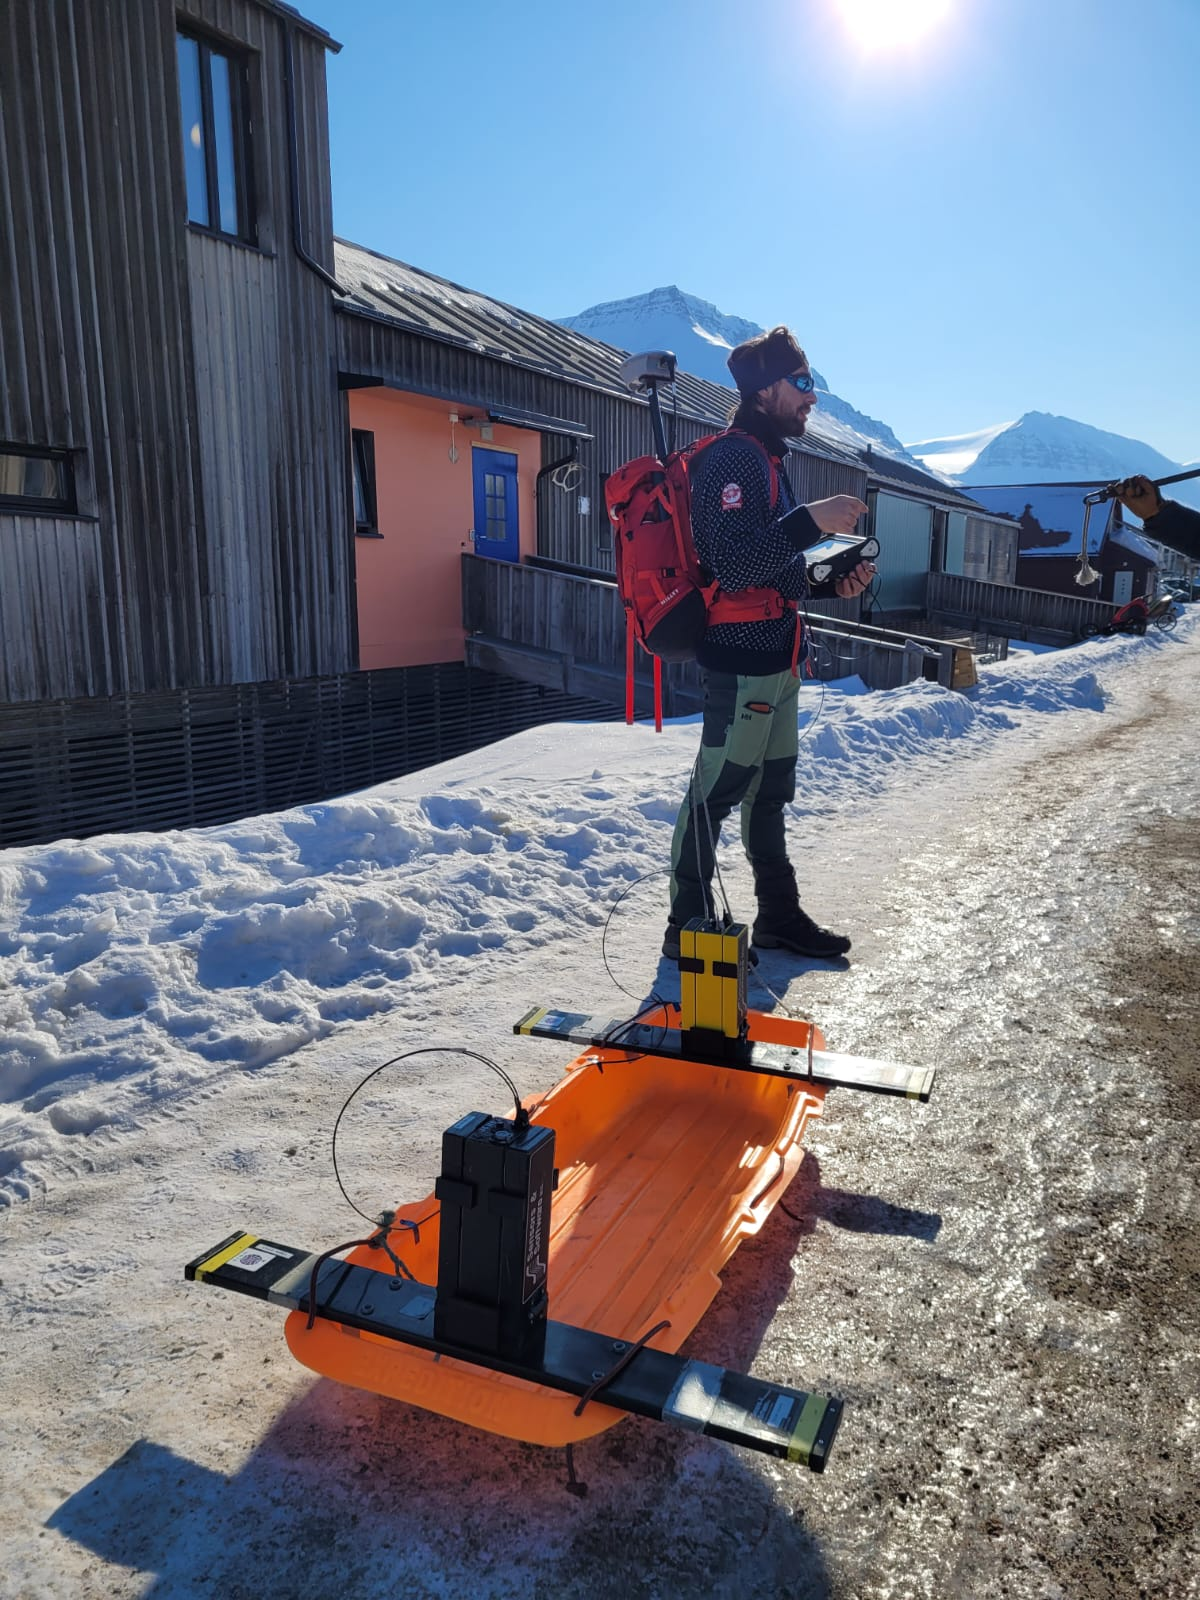
\includegraphics[width=1.0\linewidth]{Images/00_Methodology/PictureGunnhild.jpg}
    \caption{GRP setup used for the survey during the tests (see \ref{Subsection:TestSurvey}) realised in the main street of Longyearbyen. \emph{Photo : Gunnhild Næss - UNIS}}
    \label{fig:PictureGunnhild}
\end{figure}

\subsection{Test survey} \label{Subsection:TestSurvey}

\subsection{Field work organisation}


\paragraph{Site description} \label{Paragraph:SiteDescription}

\paragraph{Geology}

\begin{figure} [H]
    \centering
    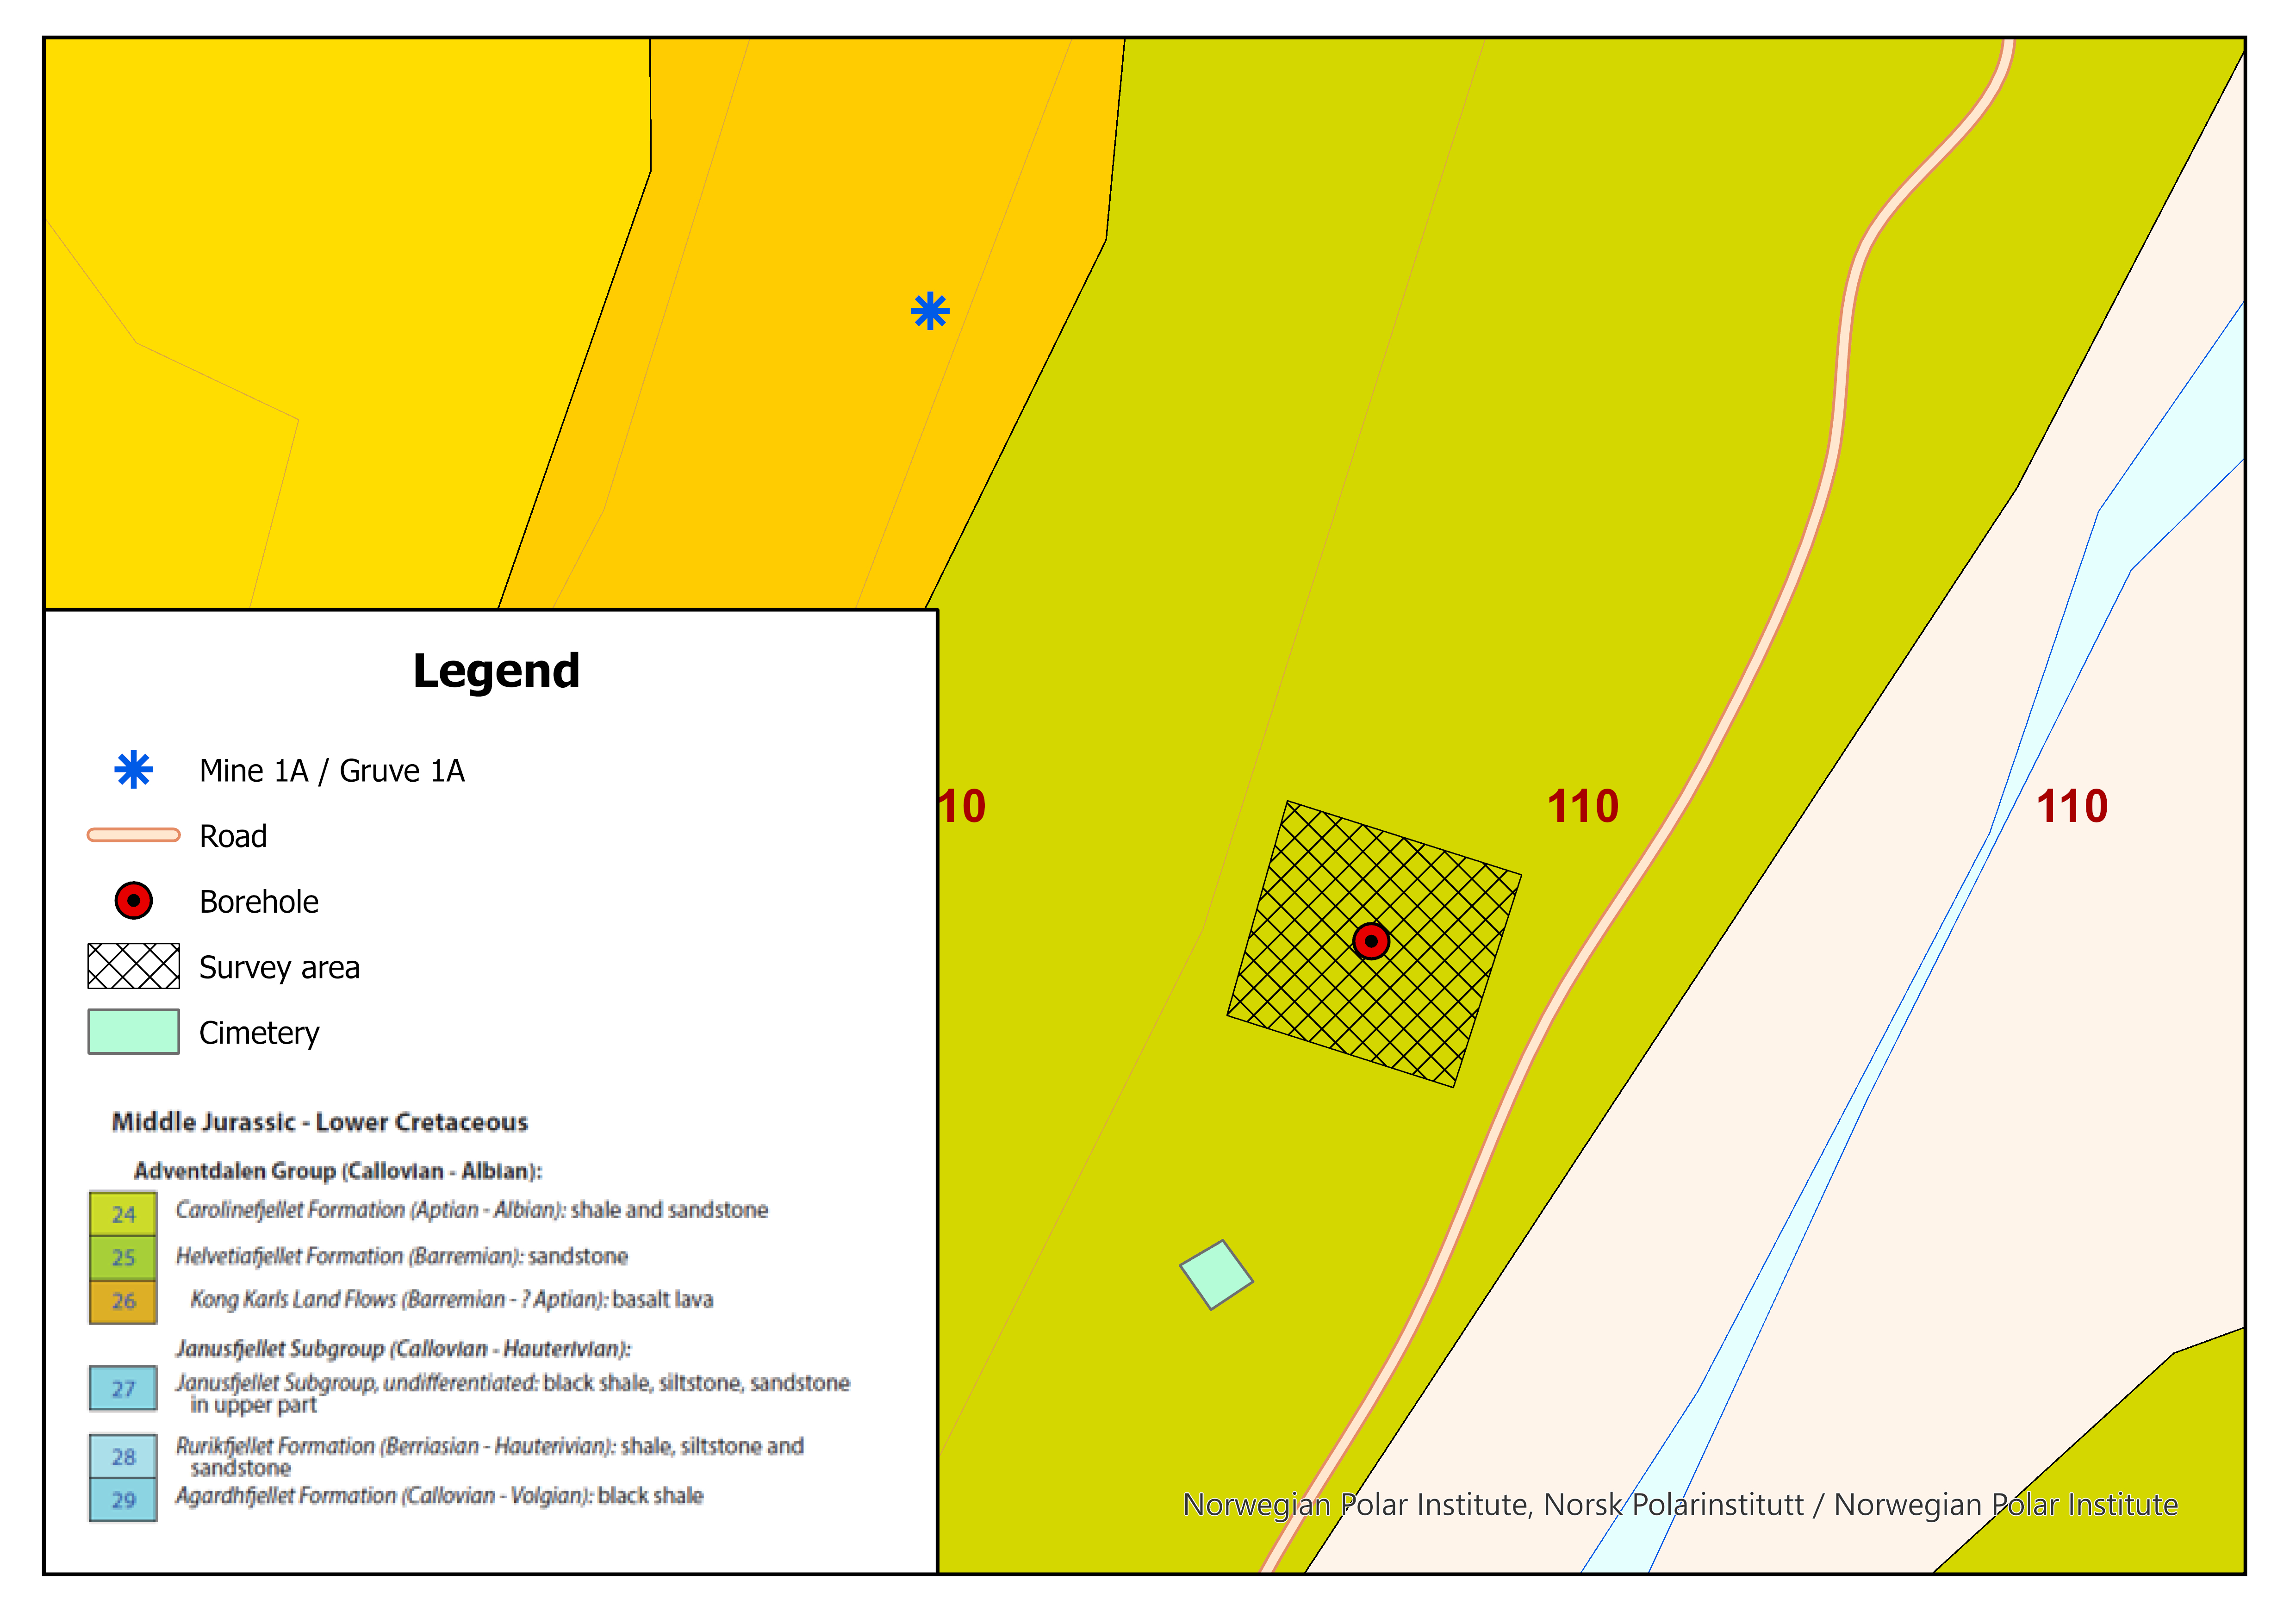
\includegraphics[width=\linewidth]{Images/00_Methodology/GeologicalSituationMap.jpg}
    \caption{Geological background under the survey area \cite{Atakan2015GeoscienceSvalbard}}
    \label{fig:GeologicalBackground}
\end{figure}

\paragraph{Weather conditions}

\paragraph{Safety consideration}

\paragraph{Planned grid}


\subsection{Processing}